\documentclass[12pt]{article}
\usepackage[margin=1in]{geometry}
\usepackage{blindtext}
\usepackage{ragged2e}
\usepackage{csquotes}
\usepackage{graphicx}
\usepackage{rotating}
\usepackage{wrapfig}
\usepackage{subcaption}
\usepackage{float}
\usepackage{amsmath,amsthm,amssymb}
\usepackage{setspace}
\usepackage{lscape}
\usepackage{caption}
\usepackage{subcaption}
\usepackage[utf8]{inputenc}
\usepackage{threeparttable}
\usepackage{pdflscape}
\usepackage{xcolor}
\usepackage{pgfplots}
\usepackage{tikz}
\usepackage{soul}
\usepackage{natbib}

\begin{document}

\begin{center}
Kaleigh Strohl \\
ECON833: Problem Set 8 \\
Fall 2021
\end{center}

Climate change and the future of our planet has become a highly debated topic. Focus has turned towards what corporate businesses can do to minimize the negative externalities they generate from running their companies (i.e. pollution, material waste, deforestation.) But for companies, altering their business model to accommodate for such demands is costly, especially when their current business model is highly profitable. Instead, they try to compensate for these externalities by vowing to take outside action to offset the damage they've created. One of those methods is pledging to save forests, advocate for the preservation of national parks, or plant a minimum level of trees in a desired location. While this is encouraging, doing so poses explicit and implicit costs to the company since they now have to invest in items outside of their business for the good of society. How do they make this decision? Is it worth it? Are the actions they take enough to fix the damage they've caused?

Let's say there's a social planner for this society who decides what is the optimal level of \enquote{green} investment each period, here in terms of land use. Their goal is to maximize utility from the level of consumption given an initial allocation of land. Land consumption (continuous) can be used for either green investment purposes or business purposes, but there are differing returns to each. Additionally, the social planner is constrained by the total allocation of land. \\
\begin{enumerate}
	\item Population of Agents
	\begin{itemize}
		\item We're modeling the decisions of the social planner on behalf of firms.
	\end{itemize}
	\item Preferences	
	\begin{itemize}
		\item The social welfare function is going to be concave function in an infinite horizon problem. Given that climate change is a ongoing concern, it cannot be assumed that we can predict when the planet is in an ideal shape or, adversely, when the planet is damaged past the point of fixing. So, the social planner needs to make these decisions for as long as possible to prevent the planet from being harmed. 
	\end{itemize}
	\item Productive Technology
	\begin{itemize}
		\item The social planner is given an initial amount of land, \(Z_0\), that they must decide how to allocate over time. Whatever they allocate today (towards either \enquote{green} or businesses purposes) cannot be used tomorrow - investment is irreversible. Let \(c_t\) be the amount of land consumed today for green investment and \(x_t\) be the amount of land consumed today for business purposes. The amount of land available tomorrow is going to be whatever is left over after the decisions made today:  
		\begin{equation}
			Z_{t+1} = Z_t - c_t - x_t
		\end{equation}
	\end{itemize}
\newpage
	\item Information Technology
	\begin{itemize}
		\item The social planner knows the initial allocation of land at period 0 and the returns to investment in either option. Given the welfare function is an increasing concave function, this suggests diminishing marginal returns to both options of investment. But the current social environment wants to encourage green investment each period, so any allocations not used for these purposes are going to be discounted since they are not directly contributing to the natural environment. Let \(\alpha\) be a parameter between 0 and 1 that identifies the utility weight for decisions to invest in the business over the environment. The parameter is exogenous and determined in period 0. If \(\alpha\) is closer to 1, then society does not care as much about the planet and is indifferent to where the social planner allocates land. If \(\alpha\) is closer to 0, then society cares a lot about the planet and is highly discouraged when the social planner doesn't allocate land to the natural environment each period. (When closer to 0, the parameter acts as a penalty.) Given preferences and this information, the social welfare function is: 
		\begin{equation}
			u(c_t) + \alpha u(x_t)
		\end{equation}
	\end{itemize}
	\item Enforcement Technology
	\begin{itemize}
		\item As previously mentioned, the decisions the social planner makes today cannot be reversed tomorrow.
	\end{itemize}
\end{enumerate}

\noindent Formally, the problem is: 
\begin{subequations}
	\begin{alignat}{4}
		&\max_{c_t, x_t} \sum_{t=0}^{\infty} \beta^t \cdot [u(c_t) + \alpha u(x_t)]\\
		&\text{subject to} &      & Z_{t+1} = Z_t - c_t - x_t \\
		&                  &      & Z_t > 0 \\
		&                  &      & c_t \geq 0 \\
		&                  &      & x_t \geq 0 \\
		&                  &      & 0 \leq \alpha \leq 1 \\
	\end{alignat}
\end{subequations}

\noindent State variables: \(Z_t\) \\
\noindent Control variables: \(c_t, x_t\)
\newpage
\noindent Bellman Equation: 
\begin{equation}
	\max_{c, x} u(c) + \alpha u(x) + \beta V(Z')
\end{equation}
\begin{center}
	subject to \(Z' = Z - c - x\)
\end{center} \\
\noindent Lagrangian:
\begin{equation}
	L = \max_{c_t, x_t} \sum_{t=0}^{\infty} \beta^t \cdot u(c_t) + \alpha u(x_t) + \sum_{t=0}^{\infty} \lambda_t (Z_t - c_t - x_t - Z_{t+1}) + \sum_{t=0}^{\infty} \phi_t c_t +  \sum_{t=0}^{\infty} \gamma_t x_t
\end{equation} \\
\noindent FOCs: 
\begin{equation}
	c_t: \qquad \beta^t u'(c_t) - \lambda_t + \phi_t = 0
\end{equation}
\begin{equation}
	x_t: \qquad \beta^t \alpha u'(x_t) - \lambda_t + \gamma_t = 0 
\end{equation} \\
\noindent Given a concave utility function, Inada conditions are met and the Lagrangian multipliers are equal to zero. Combining FOCs, we have an equation that determines the optimal level of \(x_t\) after choosing \(c_t\): 
\begin{equation}
	u'(c_t) = \alpha u'(x_t)  
\end{equation} \\
\noindent We can also construct Euler equations for \(c_t\) and \(x_t\):
 
\begin{equation}
	u'(c_t) = \beta u'(c_{t+1})
\end{equation}
\begin{equation}
	u'(x_t) = \beta u'(x_{t+1})
\end{equation}

\newpage
\noindent Visualizations of this model are included above. As we can see on the left, the level of social utility increases with the level of land allocation at a decreasing rate. But utility is negative, which seems like an issue that I do not know how to resolve at this moment. When I changed the alpha parameter, the closer the value was to 1, the more negative the y-axis values became, which is what was expected. On the right, we see that the level of \enquote{green} investment is increasing with the amount of land allocated.

\begin{figure}[!tbp]
	\caption{Visual Output}
	\begin{subfigure}[b]{0.45\textwidth}
		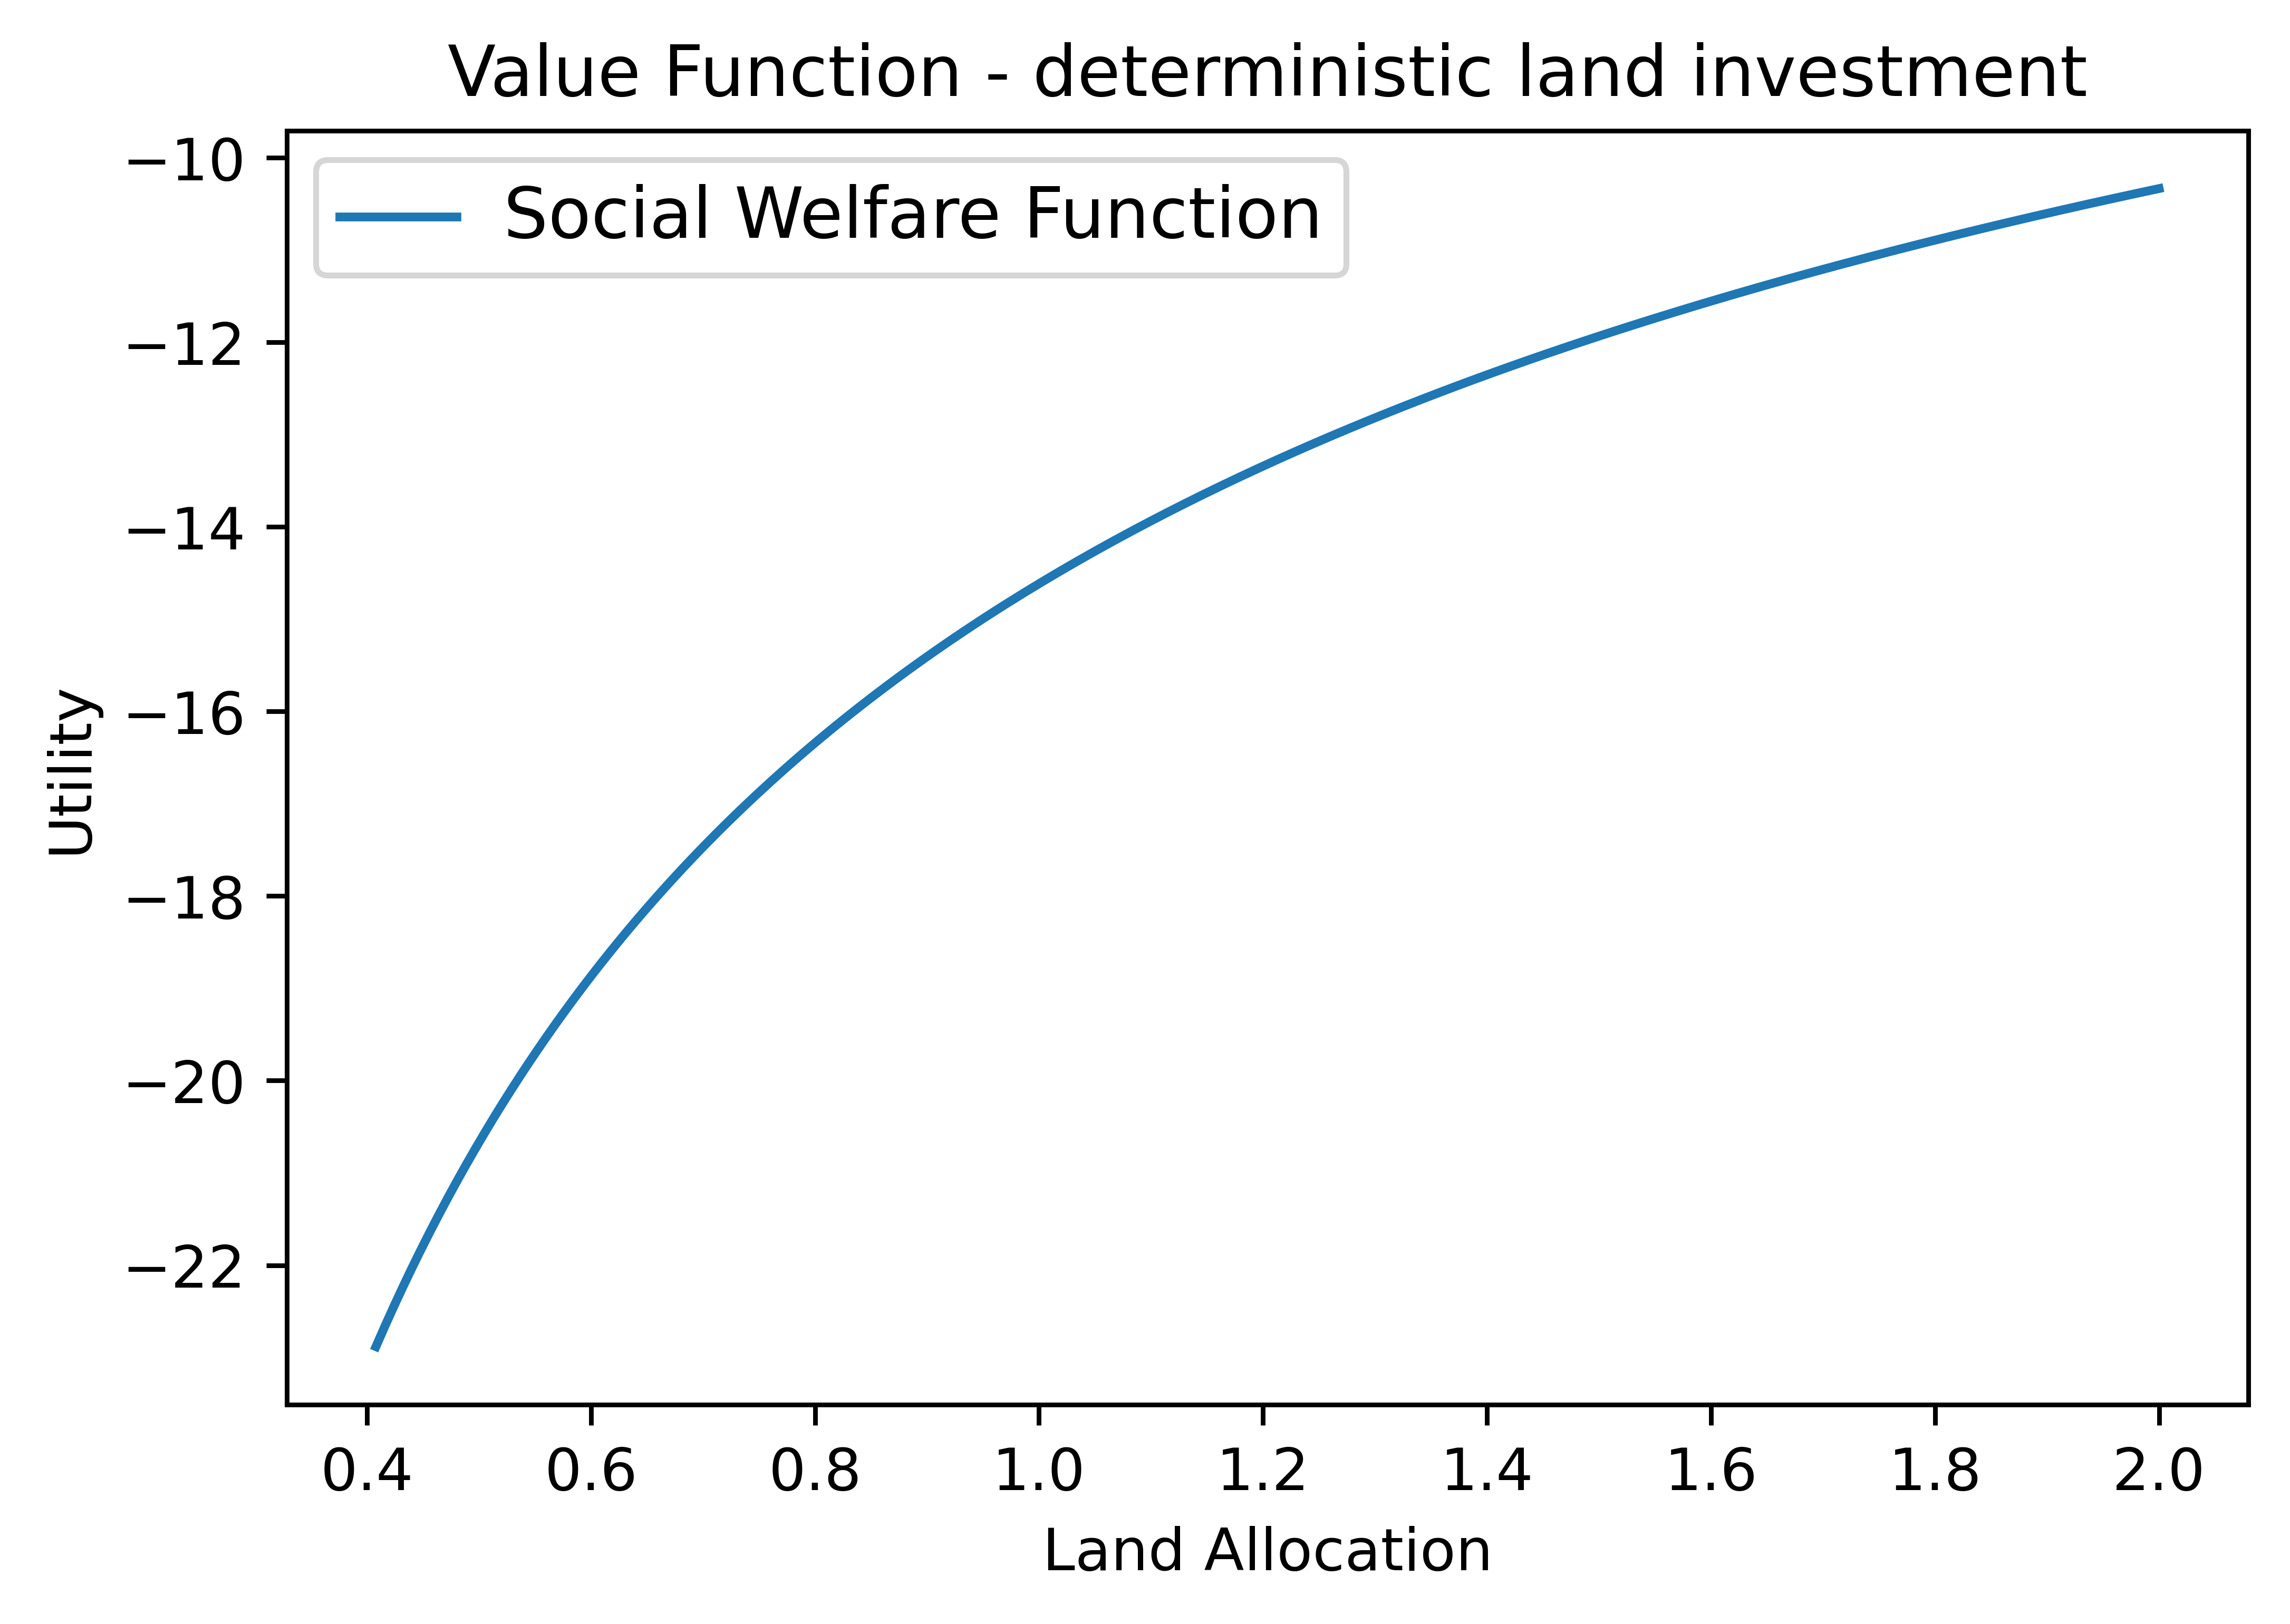
\includegraphics[width=\textwidth]{PS8_VF.png}
		\caption{Value Function}
	\end{subfigure}
	\hfill
	\begin{subfigure}[b]{0.45\textwidth}
		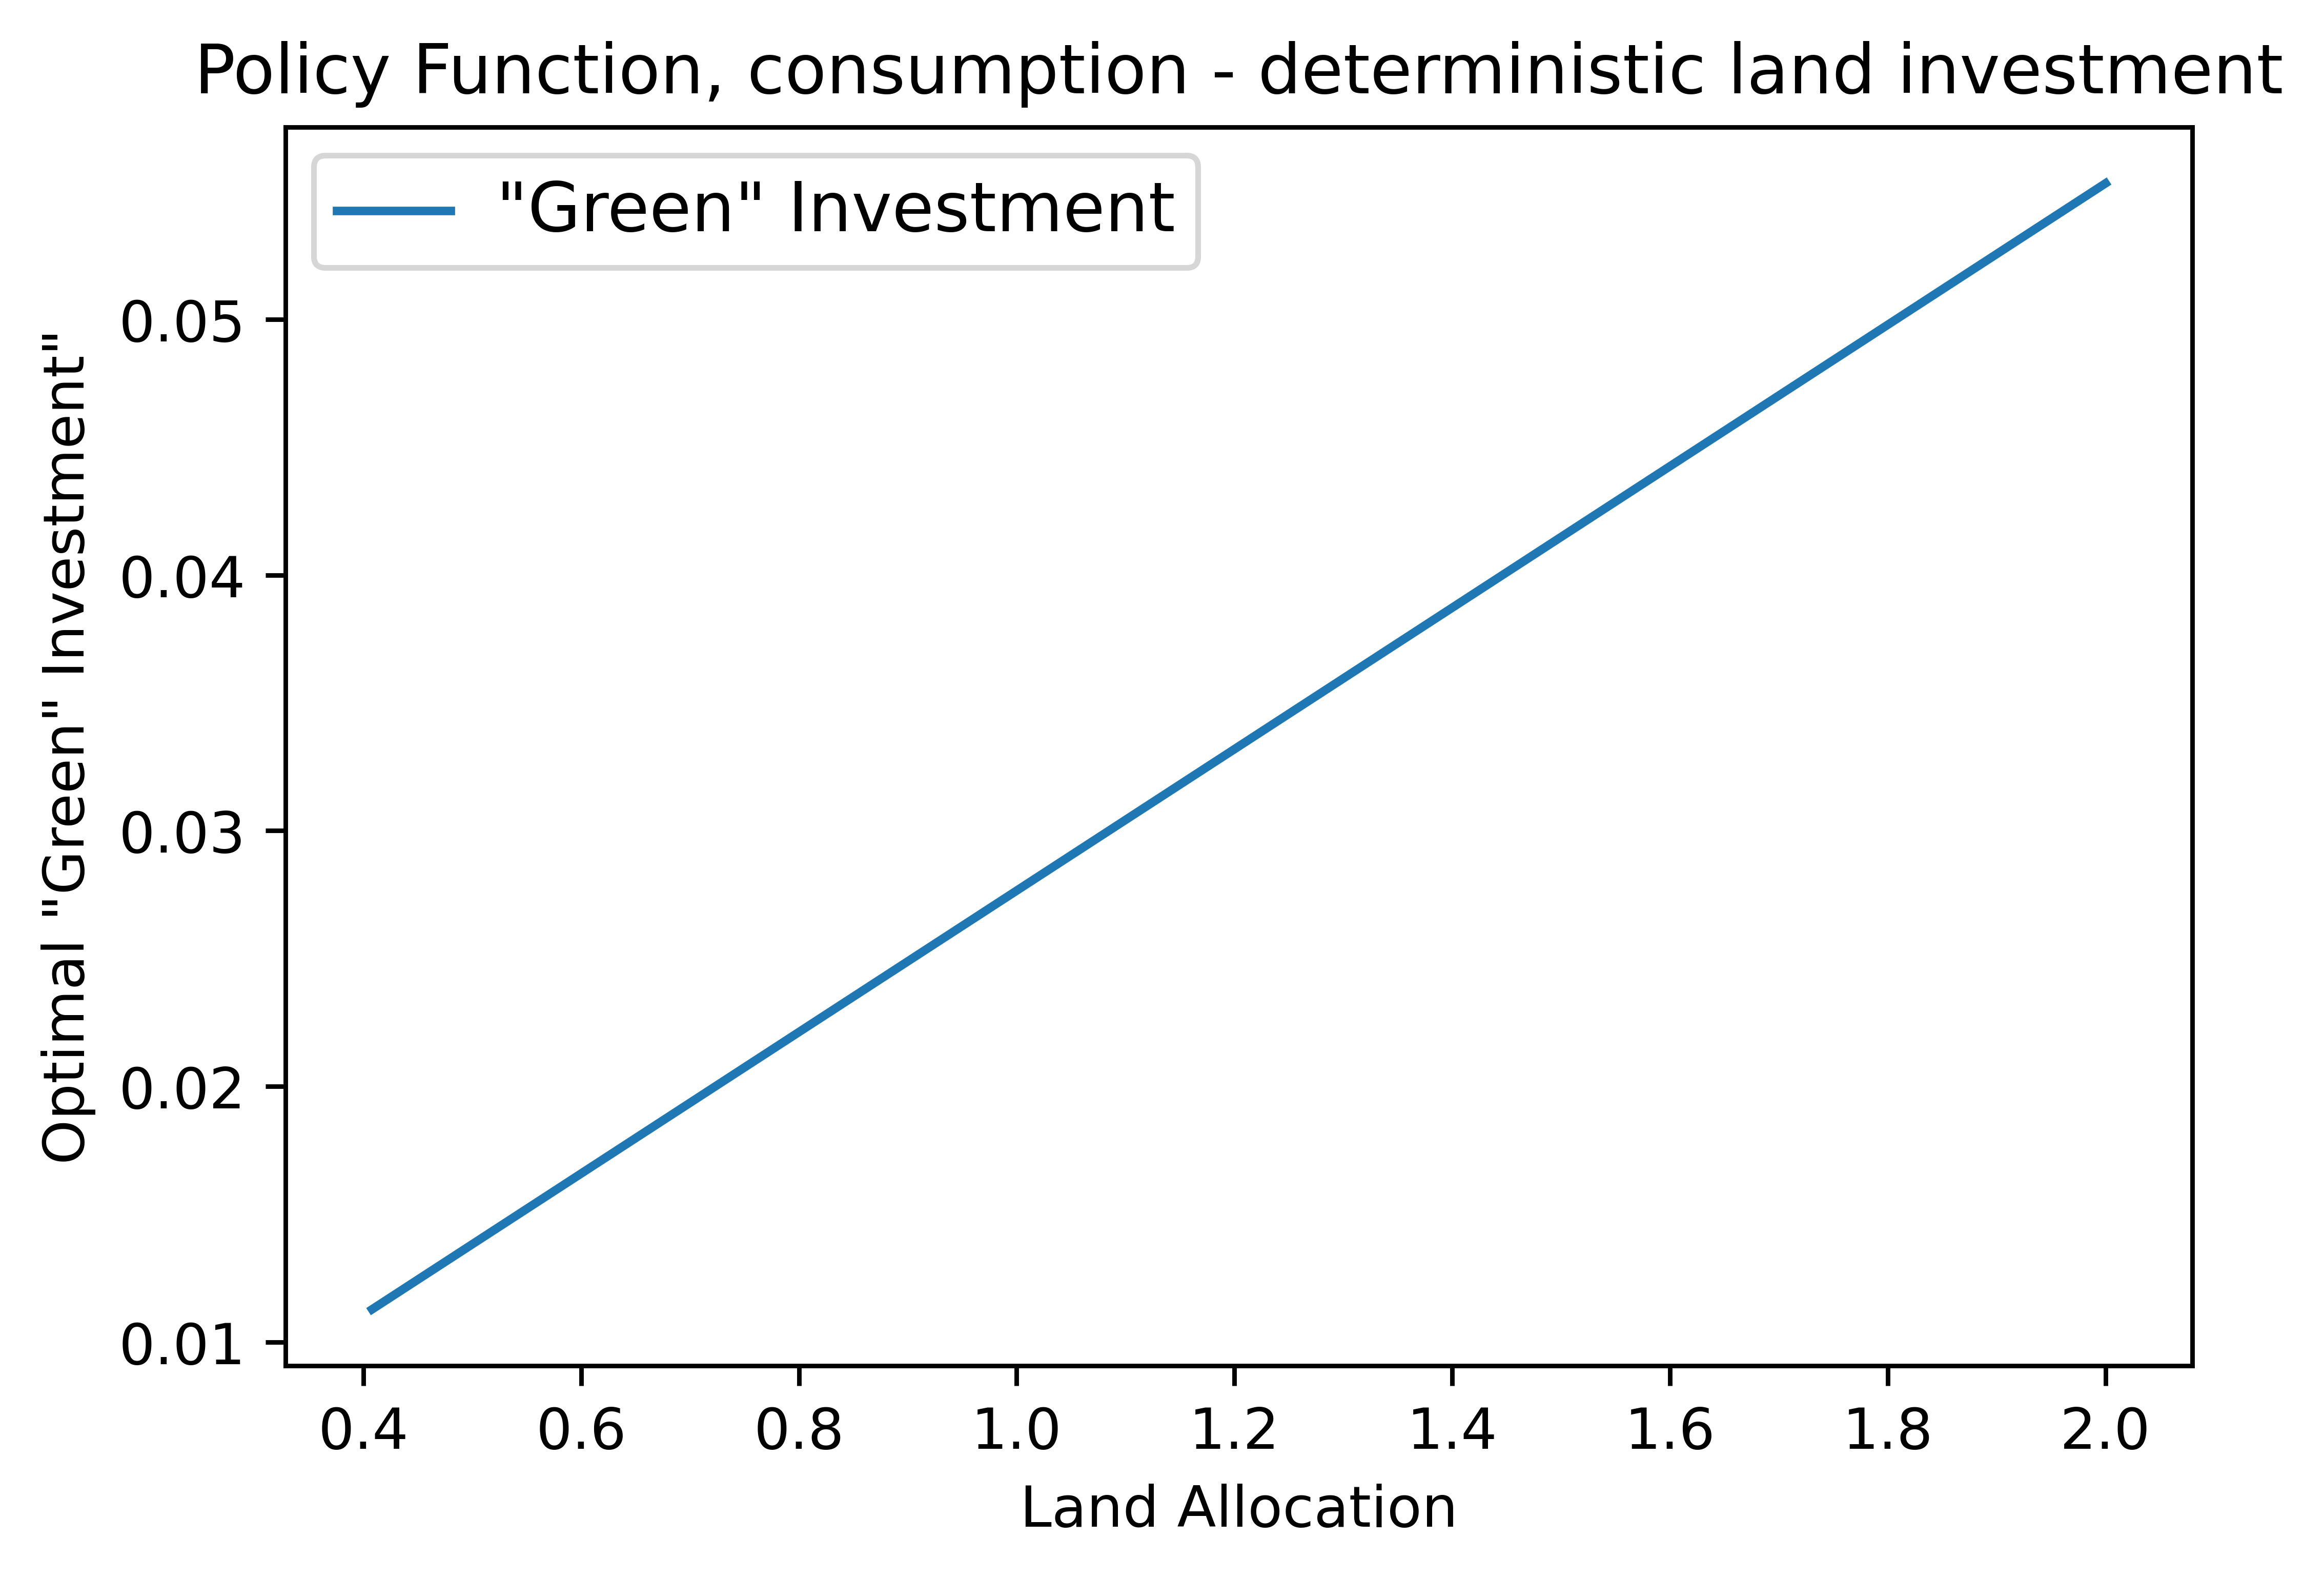
\includegraphics[width=\textwidth]{PS8_PF.png}
		\caption{Policy Function}
	\end{subfigure}
\end{figure}

\end{document}